\chapter{Calculation of voltage distribution in TPC}
\label{chapter:wirefield}
Electrostatic simulation for understanding the electric field distribution in the detector has been long evaluated. There are many software package that numerically solve this Poisson Partial Differential equation(PDE) problem using Finite Element Analysis(FEA) Method for given boundary condition. The common used softwares are, Matlab \& Simulink, Elmer FEM solver, Maxwell, Comsol Multiphysics, etc. However, the cost of solving the exact problem using FEM is expensive, especially for 3 dimensional problems, or to get a more precise solution. The reason for is the size of problem grow very quickly as problem goes to 3d. 
However, this problem can be simplified in the detectors that are composed with simple reducible parallel segment, for example, most of the wire chambers, parallel TPCs. In this section we are going to talk about a method to estimate the electric field in these detectors.

\section{Parallel-component detectors}
The electric field equation of the space is solved by Poisson equation:
\begin{align}
&\nabla^2\Phi = -\rho/\epsilon 
\end{align}
where $\rho = 0$, expect for on the components or on the boundary.
Suppose we have a detector with $n$ parallel components. They are sequently residing in the space. From top to bottom is component $1,2, ... n$. The thickness of the $i$th component is $d_i$. The position of the $i$th component is $z_i$   
For a detector that is composed with simple parallel components, for example, wire planes, etched metal planes, if each component is distant away from the other components, we can separate the solutions for each components by dividing the problem to a Poisson electric field equation with one component in each space and the voltage boundary condition on the conjunction.\\
Normally because of it is hard to directly control the charge distribution of each component, with most high voltage power supplies, the normal method to operate is to have a desirable voltage potential, we assume the voltage on the $i$th component is $V_{,i}$. However, because of the component, for example, wire plane, etched metal plane is not 100\% occupying the plane, the voltage potential of the void plane is normally different of the voltage on the component. We assume the average potential of the $i$th plane, the effective voltage of the $i$th component is $V_{0,i}$, like in fig: \ref{fig: parallel dec}.
\begin{figure}
\centering

\includegraphics[width=.5\textwidth]{blank.jpg}
\caption{An example of a detector with parallel components. The actual voltage of the $i$th component is $V_{,i}$, the effective voltage of the $i$th component is $V_{0,i}$, the effective electric field on the top side of the $i$th component is $E_{up,i}$, the effective electric field on the bottom side of the $i$th component is $E_{down,i}$, etc.}
\label{fig: parallel dec}
\end{figure}
\\
Because of there is no space charge between two neighbor components, the average electric on a plane parallel to the detector components between two neighbor components should be a constant. We call the average effective electric field on the top side of the $i$th component, $E_{up,i}$, the average effective electric field on the bottom side of the $i$th component is $E_{down,i}$. We should have
\begin{align}
\boldsymbol{E}_{down, i}= \boldsymbol{E}_{up, i+1}.
\end{align}
\\
If the detector is big and infinite in size in $x$ and $y$ direction, or within each component there is a periodic pattern on $x$ and $y$ direction, from Gaussian's law, we can easily get that on the top and bottom boundary, which is far away from the detector components, the electric field only has $z$ direction components. 
\begin{align}
\boldsymbol{E}|_{top, i} & = E_{up, i} \boldsymbol{e_z}\\
\boldsymbol{E}|_{bottom, i} & = E_{down, i} \boldsymbol{e_z}
\end{align}
\\
The relation ship between the effective voltage $V_{0,i}$ and the effective electric field on the top and bottom of detector component $E_{up,i}$, $E_{down,i}$ is 
\begin{align}
E_{down, i}* (z_{i+1}-z_{i}-d_{i}) = V_{i+1}-V_{i}.
\end{align}
If the thickness of each component $d_i$ is small, the equation can be simplified as
\begin{align}
E_{down, i}* (z_{i+1}-z_{i}) = V_{0,i+1}-V_{0,i}.
\end{align}
Then we take a look at a section with one component. We can separate the electric field in the space $\boldsymbol{E}(\boldsymbol{x})$ into two parts,  
\begin{align}
\boldsymbol{E}(\boldsymbol{x}) = E_{\parallel} \boldsymbol{x} + \boldsymbol{E}_{else}(\boldsymbol{x})
\end{align}
where the uniformed electric field along the x axis with magnitude $E_{\parallel}=\frac{1}{2}(E_{down, i} + E_{up, i})$. We notice that this part has no contribution to the net charge on the detector component. Thus, its contribution to the difference between the actual voltage on the detector components and the effective voltage along the plane where the detector components is. The rest part of the electric field is $E_{else}$. On the boundary on the top and the bottom of the section, it has new boundary conditions, 
\begin{align}
\boldsymbol{E}|_{top, \infty, i}  & = (E_{up, i}-\frac{1}{2}(E_{down, i} + E_{up, i})) \boldsymbol{e_z}, \\
\boldsymbol{E}|_{bottom, \infty, i}  & = (E_{down, i}-\frac{1}{2}(E_{down, i} + E_{up, i})) \boldsymbol{e_z}.
\end{align}
\\
The solution of this problem with the detector component geometry and the new boundary condition is $\boldsymbol{E}_{else}'$. 
\\
If the detector component is thin, then the two separate solutions have the same boundary condition, which means $\boldsymbol{E}_{else}' = \boldsymbol{E}_{else}$. 
The electric field scales with the potential in the space. If the solution for the potential and the electric field are $V(\boldsymbol{x})$, $\boldsymbol{
E}_{\boldsymbol{x}}$. The solution with the same space and $a$ times the value of the electric field on the boundary are $a V(\boldsymbol{x})$, $a \boldsymbol{
E}(\boldsymbol{x})$. Since from previous discussion we know that $E_{up, i}-E_{down,i}$ component has more contribution to the solution than $E_{up, i}-E_{down,i}$ component. So we have
\begin{align} 
\Delta V & = V_{,i}-V_{0,i} \\
		 & \propto E_{up, i}-E_{down,i}.
\end{align}
If the detector component has period conditions on the $x$, $y$ plane with dimension $p$, the electric field and the potential in the space scale with this dimension $p$. The solution with in a space that is $a$ times larger and the same value of the electric field are $V_{new}(a \boldsymbol{x}) = V(\boldsymbol{x}) $, $\boldsymbol{
E}_{new}(a \boldsymbol{x}) = \frac{1}{a}\boldsymbol{
E}(\boldsymbol{x})$. So we have
\begin{align} 
\Delta V & \propto p.
\end{align}
So we can write 
\begin{align}
\Delta V \approx G(E_{up, i}-E_{down,i})p.
\end{align}
Grid factor $G$ is a function of the geometry of the detector component. \\
From Maxwell equations, we got the charge distribution on the detector components should follow 
\begin{align}
 \nabla \bullet \boldsymbol{E} = \rho/ \epsilon.
\end{align}
So the charge on the detector component for a given area is 
\begin{align}
d\rho/ds = \epsilon E
\end{align}
Because of the parallel component is usually not zero, so the charge distribution on the top and bottom side of the detector component is usually different. For a given area on the surface of the component, the charge difference between the top and the bottom side is roughly $\rho = \epsilon_0(E_{up, i}+E_{down, i})$.  
\\
The force on the detector component for a given area is 
\begin{align}
dF/ds = \rho E_{external}
\end{align}





\subsection{A single grid plane}
The most common detector component is single grid plane. For a grid that is consist of infinitely thin wires along $y$ axis on the $z=0$ plane. which are uniformly separated by distance $a$, like fig \ref{fig: single wire}. Assuming the electric field on the top and bottom boundary is symmetric and the values are
\begin{align}
z \ll 0:& \quad  \frac{1}{2}E_{dif}\\
z \gg 0:& \quad -\frac{1}{2}E_{dif}
\end{align}
The solution for this problem is 
\begin{align}
V(\boldsymbol{x}) = \frac{1}{4 \pi} a E_{dif}\ln [2(\cosh\frac{2 \pi z}{a}-\cos\frac{2 \pi x}{a})].
\end{align}
The effective voltage potential on the $z=0$ plane is 0. 
If the dimension of the wires $r$ is not negligible,  the potential on the wire should be 
\begin{align}
V(x) &\approx \frac{1}{4 \pi} a E_{dif}\ln [2(1+(\frac{2 \pi z}{a})^2/2-1+(\frac{2 \pi x}{a})^2)/2] \\
& = \frac{1}{2 \pi} a E_{dif}\ln \frac{2 \pi r}{a},
\end{align}
where $r^2 = z^2 +x^2$.
So the grid factor $G$ is 
\begin{align}
G = \frac{1}{2 \pi} \ln \frac{2 \pi r}{a}
\end{align}
And the average electric field on the surface of the wire $E_{av}$ is 
\begin{align}
E_{av}= E_{dif}\frac{a}{2 \pi r}
\end{align}
\begin{figure}
\centering

\includegraphics[width=0.5\textwidth]{blank.jpg}
\caption{The geometry of a single grid plane, with spacing $a$.}
\label{fig: single wire}
\end{figure}
the charge on the wire in a uniformly electric field $E_{\parallel}$ is 
\begin{align}
d\rho/ds = \epsilon E_{\parallel} \cos \theta
\end{align}
So the overall charge on the wire should roughly be
\begin{align}
d\rho/ds & \approx \epsilon (E_{av}+E_{\parallel} \cos \theta) 
\end{align}
The transparency of the grid $T$ is the probability that an electron from infinity distance from the bottom of the grid drift passing the grid. The grid gains full transparency if the sign of the charge on the grid wires are negative everywhere, which is
\begin{align}
E_{av}-E_{\parallel} \geq & 0 \\
-(E_{up, i}-E_{down,i})\frac{a}{2 \pi r} - \frac{1}{2}(E_{up,i}+E_{down,i}) \geq & 0 \\
\frac{E_{down,i}}{E_{up,i}} \geq & \frac{a + \pi r}{a - \pi r}
\end{align}
%%%This part does not have consistent mathematical result compare to the previous session.
% The analytic solution of a single plate with different spacing between wires but same periodic pattern is 
% \begin{align}
% V(\boldsymbol{x}) & = \sum_{i=1}^n E_{i} \frac{a}{4 \pi} \ln [2(\cosh \frac{2 \pi z}{a} - \cos \frac{2 \pi (x-a_{i})}{a})] \\
% E_{top, \infty} & = -E_{bottom, \infty} = \frac{1}{2}\sum_{i=1}^{n} E_{i} \\
% V_{j} & \approx E_{j} \frac{a}{2 \pi} \ln \frac{2 \pi r_{j}}{a} + \sum_{i\neq j}^{n} E_{i} \frac{a}{4 \pi} \ln [2(1 - \cos \frac{2 \pi (a_{j}-a_{i})}{a})] 
% \end{align}
% where $r_{j}$, $a_{j}$, $V_{j}$ are the radius, location, potential on the $j$th wire. \\
% For simple case $n = 2$, where which means $r_{1}=r_{2}=r, V_{1}=V_{2}= V_{wire}$,
% \begin{align}
% V_{wire} & \approx E_{dif}\frac{a}{4 \pi} \ln \frac{2 \pi r}{a} + E_{dif} \frac{a}{8 \pi} \ln [2(1 - \cos \frac{2 \pi (a_{1})}{a})] \\
% G & \approx \frac{1}{4 \pi} \ln \frac{2 \pi r}{a} + \frac{1}{8 \pi} \ln [2(1 - \cos \frac{2 \pi (a_{1})}{a})] \\
% &\approx \frac{1}{4 \pi} \ln \frac{2 \pi r}{a} \quad where \quad a_1 = \frac{a}{2}
% \end{align}

\subsection{A meshed grid plane}
A meshed grid contains wires along different directions. A simple meshed grid is consist of two single grid planes, which has wires along two perpendicular directions. \\
The grid factor of this is calculated by simulations. We put up a geometry that has the smallest cell of periodic pattern, fig: \ref{fig: comsol geo}.
The grid planes location in the middle. The top and bottom plane of the cell box are both $1 cm$ from the grid plane. They as well as the wire grid itself are assign with separate voltages $V_{top}$, $V_{bottom}$ and $V_{grid}$. $V_{top} = V_{bottom}$ to make the cell symmetric. $E_{top}$ and $E_{bottom}$ are read from the result. The effective voltage on the grid plane $V_{0}$ is
\begin{align}
V_{0}= V_{top}- E_{top}* 1 cm.
\end{align}
The grid factor $G$ is
\begin{align}
G = \frac{V_{grid}-V_0}{2 E_{top}}
\end{align}
The results of grid factor is in fig: \ref{fig: g factor meshed}. The curve can be roughly approximated to 
\begin{align}
G = \frac{0.5247}{2 \pi} \ln \frac{0.5247 a}{\pi 0.7488 d},
\end{align}
which is equivalent to the result of a grid plane with wire radius a factor of $0.7488$ smaller and wire spacing a factor of $0.5247$ smaller.\\
The effect of the top bottom ratio of the electric field are also studied by simulation with $V_{top} \neq V_{bottom}$. Results in fig: \ref{fig: Etop bottom effect meshed} show that this effect is small. Thus the approximation method we used to calculate voltage in the detector is valid. 
\begin{figure}
\centering

\includegraphics[width=0.5\textwidth]{blank.jpg}
\caption{The geometry of a meshed grid plane, with spacing $a$.}
\label{fig: geo meshed}
\end{figure}

\begin{figure}
\centering
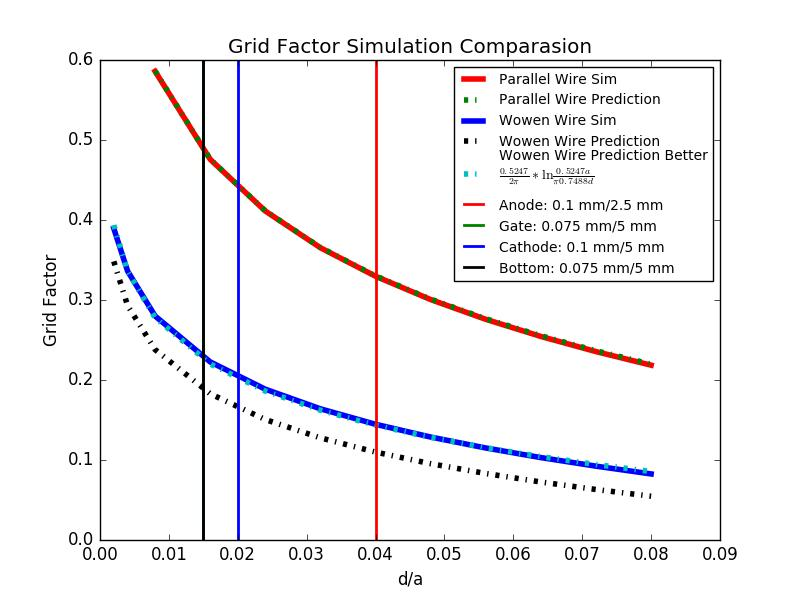
\includegraphics[width=0.5\textwidth]{Figures/A/GridFactor.jpg}
\caption{The simulation result of grid factor for equal-spaced meshed grid. }
\label{fig: g factor meshed}
\end{figure}

\begin{figure}
\centering

\includegraphics[width=0.5\textwidth]{blank.jpg}
\caption{The simulation result how much is the effect of the top bottom ratio of electric field on grid factor for equal-spaced meshed grid. }
\label{fig: Etop bottom effect meshed}
\end{figure}

\begin{figure}[h!]
  \centering
  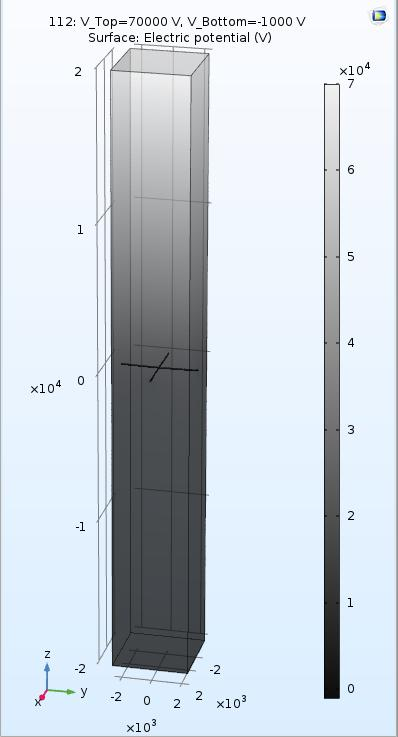
\includegraphics[width=0.5\textwidth]
  {Figures/ComsolGeo.jpg}
  \caption{A picture of Comsol simulationsimulation. }
  \label{fig: comsol geo}
\end{figure}

\subsection{etched grid with triangle, square or hexagon pattern}
Similar simulation with Comsol Multiphysics are done for etched grid with triangle, square or hexagon pattern, fig: \ref{fig: geo etched}. Results on in fig: \ref{fig: result etched grid}.  

\begin{figure}[h!]
  \centering
  
\includegraphics[width=0.5\textwidth]
  {blank.jpg}
  \caption{The geometry of an etched grid with triangle, square or hexagon pattern. }
  \label{fig: geo etched}
\end{figure}

\begin{figure}[h!]
  \centering
  
\includegraphics[width=0.5\textwidth]
  {blank.jpg}
  \caption{The grid factor of an etched grid with triangle, square or hexagon pattern. }
  \label{fig: result etched grid}
\end{figure}

\section{Deflection of the grid plane}
Since charge on the grid component are also experience the Comlomb force. And this force will deflect the grid plane. It is important for us to know the deflection of the grid planes to get a better understanding of the potential distribution in the detector. There are many different method to estimate this. Here is the most common method.
\\
This first method is called single wire calculation. For a uniformed rope with density of force per unit length $\lambda$. Assuming the tension of the end of the rope is $T$, and this tension should be the same along the rope.
\\
The curve of the rope underneath the force should balance this force with its tension, like fig: \ref{fig: sag rope}. 
\begin{figure}
\centering

\includegraphics[width=0.5\textwidth]{blank.jpg}
\caption{The sagging rope.}
\label{fig: sag rope}
\end{figure}
It follow equations,
\begin{align}
T_{1x} & = T_{2x} \\
T_{1y} - T_{2y} & = \lambda ds  
\end{align}
where $ds$ is the length of the rope between $x$ and $x'$, $ds = \sqrt{y'^2+1} dx$. Since $\frac{T_y}{T_x} =y'$, 
\begin{align}
T_{x} y'' dx = \lambda \sqrt{y'^2+1} dx.
\end{align}
The solution is a catenary curve,
\begin{align}
y & = A \cosh \frac{x}{A}, \\
A & = \frac{T_{x}}{\lambda}.
\end{align}
\\
The catenary curve can be approximated by a parabolic curve. 
\begin{align}
y & = \frac{1}{2 A}x^2
\end{align}
So we get the famous sag formula, $s$ is approximately  
\begin{align}
s = \frac{\lambda l^2}{8 T}
\end{align}
where $l$ is the total horizontal distance between the two hanging points. 
\\
For a single grid with wire diameter $d$, spacing $a$ and top bottom electric field $E_{top}$ and $E_{bottom}$. The virtual work per unit area for moving the grid plane up a distance $l$ is the changing of electric field energy, which is $\frac{1}{2}\epsilon (E_{top}^2 - E_{bottom}^2) l$. So the force density per unit area is $P = \frac{1}{2}\epsilon (E_{top}^2 - E_{bottom}^2)$. The force density per unit length $\lambda $ is 
\begin{align}
\lambda & = \frac{1}{2}\epsilon (E_{top}^2 - E_{bottom}^2) a 
\end{align}
Thus sag in the center should be,
\begin{align}
s = \frac{1}{2} \epsilon (E_{top}^2 - E_{bottom}^2) a \frac{l^2}{8 T}
\end{align}
\\
For a mesh grid with same spacing $a$ on $x$ and $y$ direction. The wire density is twice the single grid, so the force is halved.\\
%Both charge density and electric field on the wires are roughly half of the single grid plane.
So the sag in the center should be,
\begin{align}
s = \epsilon (E_{top}^2 - E_{bottom}^2) a \frac{l^2}{32 T}
\end{align}
\\
The other method is called membrane method. We treat the full grid as a part of a big membrane sphere with radius $R$. This sphere is so big that the grid plane is a small section. For easiness of discussion, let's take a circle grid perimeter with radius $R'$. The force on unit area in a membrane, pressure on the membrane is $P$ is the same as in previous discussion. The total force perpendicular to the perimeter line $F'$ along the perimeter should contain in
\begin{align}
F' \frac{R'}{R} = P \pi R'^2 .
\end{align} 
For a grid plane, like , the total number of wire ends in the circle perimeter is $2* 2 R'/a$. If each wire is tension with force $T$, the total force perpendicular to the perimeter line is
\begin{align}
F' & = \sum T_i \cos \phi_i \\
& = \sum T \frac{l_i}{2 R'}\\
& \approx 2 T \frac{\pi R'^2/a}{2 R'} \\
& = \frac{\pi T R'}{a}
\end{align}
where $\phi_i$ is the angle between the line that connect the $i$th wire end and the membrane center and the $i$th wire. $l_i$ is the length. The factor $2$ comes from each wire has two ends.
\\
So total deflection $s$ which is calculated from the geometry of the sphere is,
\begin{align}
s & = \frac{R'^2}{2 R} \\
& = \frac{a P R'^2}{2 T} \\
& = \frac{1}{2}\epsilon (E_{top}^2 - E_{bottom}^2) \frac{a l^2}{8 T}
\end{align}
\begin{figure}[h!]
  \centering
  
\includegraphics[width=0.5\textwidth]
  {blank.jpg}
  \caption{A membrane single grid plane.}
  \label{fig: membrane grid plane}
\end{figure}
\\
With similar discussion the sag of a meshed grid should be half of the single grid plane.

























\begin{figure}[h!]
  \centering
  
\includegraphics[width=0.5\textwidth]
  {blank.jpg}
  \caption{}
  \label{fig:}
\end{figure}





